%<*figvecfields>
\begin{figure}
    \centering
    \newcommand*{\subfigwidth}{.49\textwidth}
    \begin{subfigure}[b]{\subfigwidth}
        \centering
        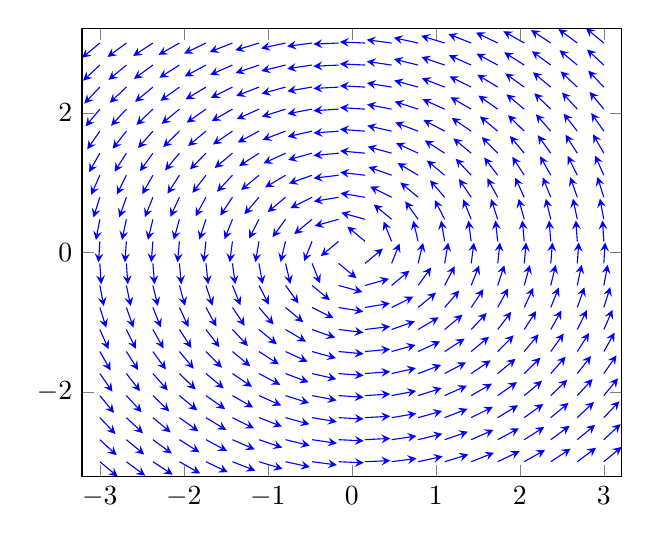
\begin{tikzpicture}
            \def\length{.5*sqrt(x^2+y^2)}
            \begin{axis}[domain=-3:3, view={0}{90}]
                \addplot3[blue, quiver={u={-y/(\length)}, v={x/(\length)}, scale arrows=0.15}, -stealth,samples=20] {0};
            \end{axis}
        \end{tikzpicture}
        \caption{
            \(
            \begin{bmatrix}
                \frac{-y}{\sqrt{x^2+y^2}} & \frac{x}{\sqrt{x^2+y^2}}
            \end{bmatrix}
            \)
        }\label{subfig:vecfield1}
    \end{subfigure}
    \vskip\baselineskip
    \begin{subfigure}[b]{\subfigwidth}
        \centering
        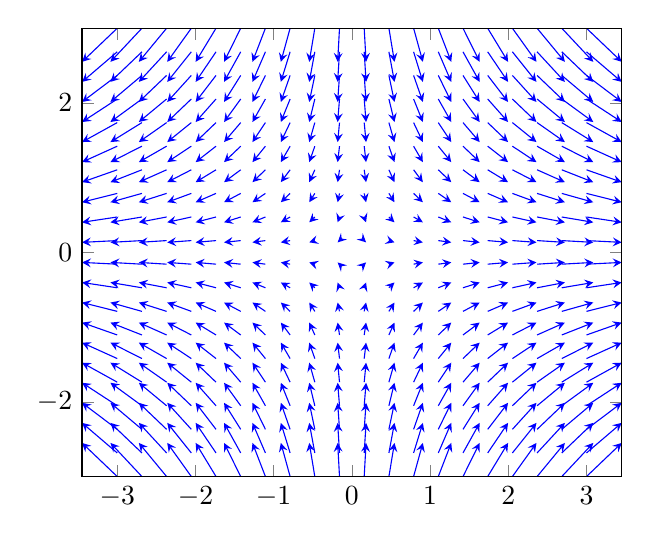
\begin{tikzpicture}
            \begin{axis}[domain=-3:3, view={0}{90}]
                \addplot3[blue, quiver={u={x}, v={-y}, scale arrows=0.15}, -stealth,samples=20] {0};
            \end{axis}
        \end{tikzpicture}
        \caption{
            \(
            \begin{bmatrix}
                x & y
            \end{bmatrix}
            \)
        }\label{subfig:vecfield2}
    \end{subfigure}
    \caption{Vector fields.}\label{fig:vectorfields}
\end{figure}
%</figvecfields>

%<*figcoordinatechart>
\begin{figure*}
    \newcommand*{\scale}{1.5}
    \centering
    \begin{tikzpicture}[thick,scale=\scale, every node/.style={scale=\scale}]
        \path[->] (0.8, 0) edge [bend right] node[left, xshift=-2mm] {$\phi_i$} (-1, -2.9);
        \draw[white,fill=white] (0.06,-0.57) circle (.15cm);
        \path[->] (-0.7, -3.05) edge [bend right] node [right, yshift=-3mm] {$\phi^{-1}$} (1.093, -0.11);
        \draw[white, fill=white] (0.95,-1.2) circle (.15cm);
    
        % Functions j
        \path[->] (5.8, -2.8) edge [bend left] node[midway, xshift=-5mm, yshift=-3mm] {$\psi^{-1}$} (3.8, -0.35);
        \draw[white, fill=white] (4,-1.1) circle (.15cm);
        \path[->] (4.2, 0) edge [bend left] node[right, xshift=2mm] {$\psi$} (6.2, -2.8);
        \draw[white, fill=white] (4.54,-0.12) circle (.15cm);
    
        % Manifold
        \draw[smooth cycle, tension=0.4, fill=white, pattern color=brown, pattern=north west lines, opacity=0.7] plot coordinates{(2,2) (-0.5,0) (3,-2) (5,1)} node at (3,2.3) {$M$};
    
        % Help lines
        %\draw[help lines] (-3,-6) grid (8,6);
    
        % Subsets
        \draw[smooth cycle, pattern color=orange, pattern=crosshatch dots] 
            plot coordinates {(1,0) (1.5, 1.2) (2.5,1.3) (2.6, 0.4)} 
            node [label={[label distance=-0.3cm, xshift=-2cm, fill=white]:$U$}] {};
        \draw[smooth cycle, pattern color=blue, pattern=crosshatch dots] 
            plot coordinates {(4, 0) (3.7, 0.8) (3.0, 1.2) (2.5, 1.2) (2.2, 0.8) (2.3, 0.5) (2.6, 0.3) (3.5, 0.0)} 
            node [label={[label distance=-0.8cm, xshift=.75cm, yshift=1cm, fill=white]:$V$}] {};
    
        % First Axis
        \draw[thick, ->] (-3,-5) -- (0, -5) node [label=above:$\phi(U)$] {};
        \draw[thick, ->] (-3,-5) -- (-3, -2) node [label=right:$\mathbb{R}^n$] {};
    
        % Arrow from i to j
        \draw[->] (0, -3.85) -- node[midway, above]{$\psi \circ \phi^{-1}$} (4.5, -3.85);
        \draw[<-] (0,-4.05) -- node[midway, below]{$\phi \circ \psi^{-1}$} (4.5, -4.05);
    
        % Second Axis
        \draw[thick, ->] (5, -5) -- (8, -5) node [label=above:$\psi(V)$] {};
        \draw[thick, ->] (5, -5) -- (5, -2) node [label=right:$\mathbb{R}^n$] {};
    
        % Sets in R^m
        \draw[white, pattern color=orange, pattern=crosshatch dots] (-0.67, -3.06) -- +(180:0.8) arc (180:270:0.8);
        \fill[even odd rule, white] [smooth cycle] plot coordinates{(-2, -4.5) (-2, -3.2) (-0.8, -3.2) (-0.8, -4.5)} (-0.67, -3.06) -- +(180:0.8) arc (180:270:0.8);
        \draw[smooth cycle] plot coordinates{(-2, -4.5) (-2, -3.2) (-0.8, -3.2) (-0.8, -4.5)};
        \draw (-1.45, -3.06) arc (180:270:0.8);
    
        \draw[white, pattern color=blue, pattern=crosshatch dots] (5.7, -3.06) -- +(-90:0.8) arc (-90:0:0.8);
        \fill[even odd rule, white] [smooth cycle] plot coordinates{(7, -4.5) (7, -3.2) (5.8, -3.2) (5.8, -4.5)} (5.7, -3.06) -- +(-90:0.8) arc (-90:0:0.8);
        \draw[smooth cycle] plot coordinates{(7, -4.5) (7, -3.2) (5.8, -3.2) (5.8, -4.5)};
        \draw (5.69, -3.85) arc (-90:0:0.8);
    \end{tikzpicture}
    \caption{Compatible coordinate charts.}\label{fig:compatcoordcharts}
\end{figure*}
%</figcoordinatechart>

%<*figcirclatlas>
\begin{figure*}
    \centering
    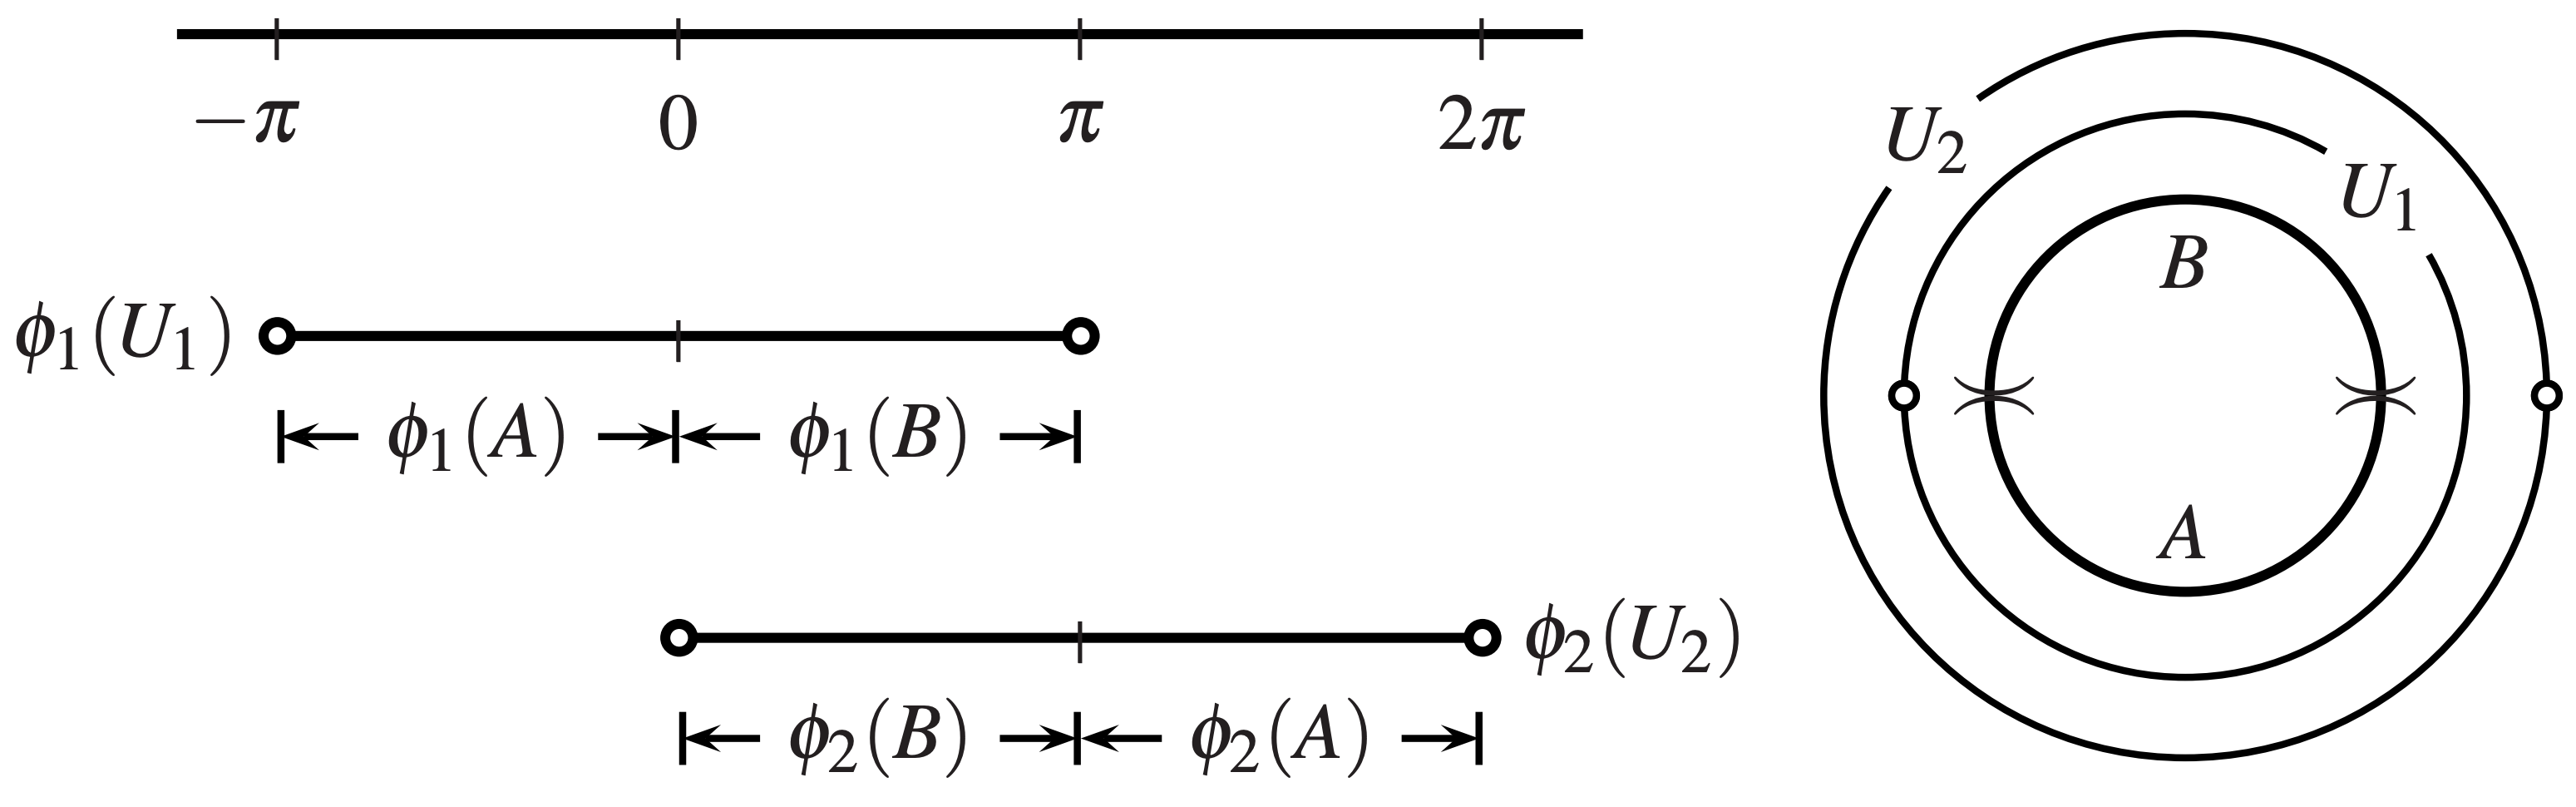
\includegraphics[width=\textwidth]{figures/chartsoncircle.png}
    \caption{Atlas of charts on the circle.}\label{fig:chartsoncircle}
\end{figure*}
%</figcirclatlas>
%<*figchartsoncirc>
\begin{figure*}
    \centering
    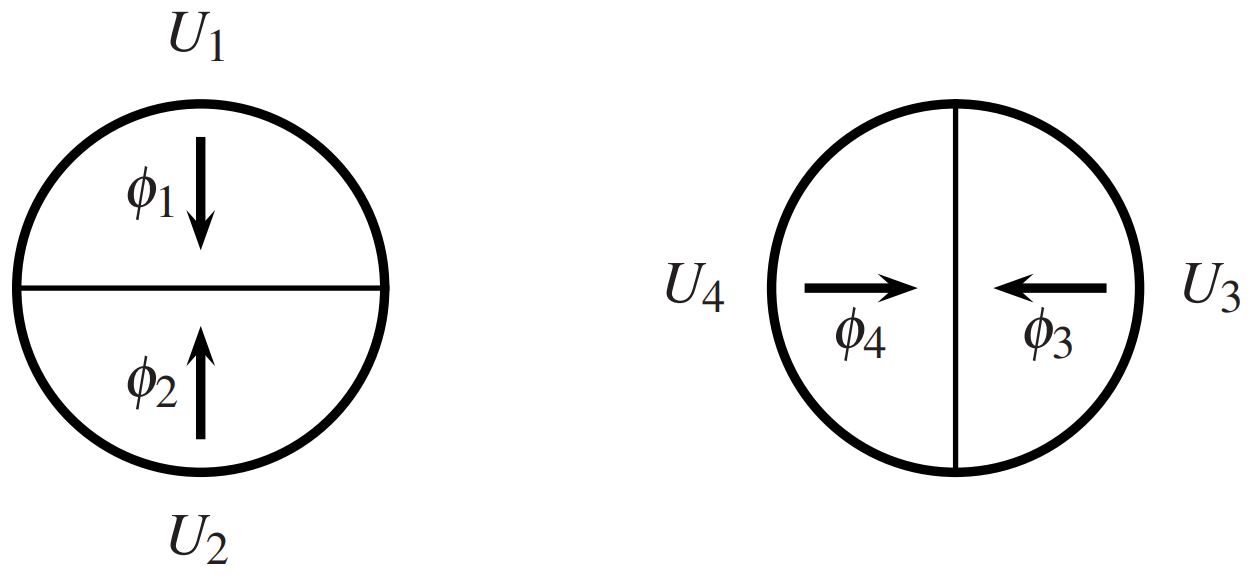
\includegraphics[width=\textwidth]{figures/xychartsoncircle.png}
    \caption{Atlas of charts on the circle.}\label{fig:xychartsoncircle}
\end{figure*}
%</figchartsoncirc>
